\documentclass[12pt,a4paper,openright,twoside]{report}

\usepackage[italian]{babel}
\usepackage[utf8]{inputenc}
\usepackage{fancyhdr}
\usepackage{float}
\usepackage{indentfirst}                        % per avere l'indentazione all'inizio dei capitoli
\usepackage{listings}                           % per il codice
\usepackage{graphicx}                           % libreria per inserire grafici
\usepackage{newlfont}                           % libreria per utilizzare font particolari, ad esempio \textsc{}
\usepackage{amssymb}                            % librerie matematiche
\usepackage{amsmath}
\usepackage{latexsym}
\usepackage{amsthm}
\usepackage{cite}
\usepackage{listings}
\usepackage{xurl}                               % per gli url nella bibliografia e per splittarli nel testo
\usepackage{hyperref}                           % per rendere gli url cliccabili
\usepackage[square,numbers,sort]{natbib}
\usepackage{xcolor}
\usepackage{caption}

\lstset{
    basicstyle=\ttfamily,
    columns=fullflexible,
    breakatwhitespace=false,
    breaklines=true,
    captionpos=b,
    keepspaces=true,
    showspaces=false,
    showstringspaces=false,
    showtabs=false,
    tabsize=4,
    aboveskip=1em,
    belowskip=1em,
    numbers=left,
    numberstyle=\ttfamily
}

\lstdefinestyle{mystyle}{
    basicstyle=\ttfamily\footnotesize,
    columns=fullflexible,
    breakatwhitespace=false,
    breaklines=true,
    captionpos=b,
    keepspaces=true,
    showspaces=false,
    showstringspaces=false,
    showtabs=false,
    tabsize=4,
    aboveskip=1em,
    belowskip=1em,
    numbers=left,
    numberstyle=\ttfamily
}

\newcommand{\source}[1]{\vspace{-10pt} \caption*{\scriptsize Fonte: {#1}} }
% \newcommand{\source}[1]{\caption*{\hfill \scriptsize Fonte: {#1}} }

\oddsidemargin=30pt
\evensidemargin=20pt

% per l'impostazione della pagina
\pagestyle{fancy}
\addtolength{\headwidth}{20pt}
\renewcommand{\chaptermark}[1]{\markboth{\thechapter.\ #1}{}}
\renewcommand{\sectionmark}[1]{\markright{\thesection \ #1}{}}
\rhead[\fancyplain{}{\bfseries\leftmark}]{\fancyplain{}{\bfseries\thepage}}
\cfoot{}

% comando per impostare l'interlinea
\linespread{1.3}

\newcommand{\xstudent}{CHRISTIAN RICCI}
\newcommand{\xsupervisor}{MORENO MARZOLLA}



\begin{document}

\pagenumbering{roman}

\oddsidemargin=25pt

\begin{titlepage}
\begin{center}
    {\Large{\textsc{Alma Mater Studiorum}}}\\
    {\Large{\textsc{Universit\`a di Bologna}}} \\
    {\textsc{Campus di Cesena}}
    % thin and big line
    \rule[0.1cm]{14cm}{0.1mm}
    \rule[0.5cm]{14cm}{0.6mm}
    DIPARTIMENTO DI INFORMATICA – SCIENZA E INGEGNERIA
    Corso di Laurea in Ingegneria e Scienze Informatiche
\end{center}

\vspace{15mm}

\begin{center}
    {\LARGE{\bf STEREO MATCHING SU GPU}} \\
\end{center}

\vspace{15mm}

\begin{center}
     \large{ Elaborato in:\\ High Performance Computing\\}
\end{center}

\vspace{20mm}
\par
\noindent

\begin{minipage}[t]{0.47\textwidth}
    {\large{\bf Relatore:\\ Prof.\\ \xsupervisor}}
\end{minipage}
\hfill
\begin{minipage}[t]{0.47\textwidth}\raggedleft
    {\large{\bf Presentata da:\\ \xstudent}} \end{minipage}
\vspace{20mm}
\begin{center}
    \large{\bf Sessione III\\ Anno Accademico 2021-2022}
\end{center}

\clearpage{\pagestyle{empty}\cleardoublepage}
\end{titlepage}

% % %%% pagina della dedica %%%
% \thispagestyle{empty}
% \topmargin=6.5cm
% \raggedleft
% \large
% \em
% (Dedica)
% \clearpage{\pagestyle{empty}\cleardoublepage}
% \end{titlepage}

% %%% indice %%%

\tableofcontents
\rhead[\fancyplain{}{\bfseries\leftmark}]{\fancyplain{}{\bfseries\thepage}}
\lhead[\fancyplain{}{\bfseries\thepage}]{\fancyplain{}{\bfseries INDICE}}
\clearpage{\pagestyle{empty}\cleardoublepage}

\listoffigures
\clearpage{\pagestyle{empty}\cleardoublepage}

%\listoftables
%\clearpage{\pagestyle{empty}\cleardoublepage}

% \lstlistoflistings
% \clearpage{\pagestyle{empty}\cleardoublepage}

\pagenumbering{arabic}



\chapter*{Introduzione}

% imposta l'intestazione di pagina
\rhead[\fancyplain{}{\bfseries INTRODUZIONE}]{\fancyplain{}{\bfseries\thepage}}
\lhead[\fancyplain{}{\bfseries\thepage}]{\fancyplain{}{\bfseries INTRODUZIONE}}

% aggiunge la voce Introduzione nell'indice
\addcontentsline{toc}{chapter}{Introduzione}

La \textit{Stereo Vision} è un popolare argomento di ricerca nel campo della Visione Artificiale; esso consiste nell'usare due immagini di una stessa scena, prodotte da due fotocamere diverse, per estrarre informazioni in 3D. L'idea di base della \textit{Stereo Vision} è la simulazione della visione binoculare umana: le due fotocamere sono disposte in orizzontale per fungere da ``occhi'' che guardano la scena in 3D. Confrontando le due immagini ottenute, si possono ottenere informazioni riguardo alle posizioni degli oggetti della scena.

In questa relazione presenteremo un algoritmo di Stereo Vision: si tratta di un algoritmo parallelo che ha come obiettivo di tracciare le linee di livello di un area geografica. L'algoritmo in origine era stato implementato per la \textit{Connection Machine CM-2}, un supercomputer sviluppato negli anni 80, ed era espresso in \textbf{*Lisp}, un linguaggio derivato dal Lisp e ideato per la macchina stessa.

Questa relazione tratta anche la traduzione e l'implementazione dell'algoritmo in \textbf{CUDA}, ovvero un'architettura hardware per l'elaborazione parallela sviluppata da NVIDIA, che consente di eseguire codice parallelo su GPU. Si darà inoltre uno sguardo alle difficoltà che sono state riscontrate nella traduzione da *Lisp a CUDA.



\rhead[\fancyplain{}{\bfseries\leftmark}]{\fancyplain{}{\bfseries\thepage}}
\lhead[\fancyplain{}{\bfseries\thepage}]{\fancyplain{}{\bfseries INDICE}}
\clearpage{\pagestyle{empty}\cleardoublepage}
\clearpage{\pagestyle{empty}\cleardoublepage}
\chapter{Programmazione Parallela}

\lhead[\fancyplain{}{\bfseries\thepage}]{\fancyplain{}{\bfseries\rightmark}}

La programmazione parallela è un paradigma di programmazione che sfrutta l'esecuzione parallela di processori per ottenere prestazioni migliori e risultati nel minor tempo possibile. I calcoli vengono eseguiti in parallelo, ovvero vengono eseguiti simultaneamente su più processori. Questo paradigma si colloca all'interno dell'High Performance Computing (HPC), una materia che studia le tecniche e soluzioni hardware e software che facilitano l'esecuzione parallela dei calcoli.



\section{Evoluzione dei Processori}

Perché ricorrere all'esecuzione parallela per ottenere prestazioni migliori? Questa domanda trova risposta nello studio dell'evoluzione dei processori: per anni si è tenuto conto della cosiddetta ``Legge di Moore'', che ipotizza che ``il numero di transistor contenuti all'interno di un chip raddoppia ogni due anni''. Questa legge fu enunciata da Gordon E. Moore nel 1965 e spiega che effettivamente le prestazioni di un chip si raddoppiavano ogni due anni. La sua osservazione si rivelò corretta per due decenni, ma intorno agli anni 2000 questo andamento iniziò a calare. I motivi principali di questo calo sono:

\begin{itemize}
    \item La dimensione dei transistor. Il miglior modo per aumentare il numero di transistor è di renderli sempre più piccoli, ma esiste un limite fisico della grandezza minima. I transistor di oggi vanno dai 20 nm ai 3 nm;
    \item Il calore dissipato dal processore. Un processore più veloce corrisponde ad una più grande quantità di calore dissipato, che porta a problemi di instabilità nel processore.
\end{itemize}

\begin{figure}[h]
    \centering
    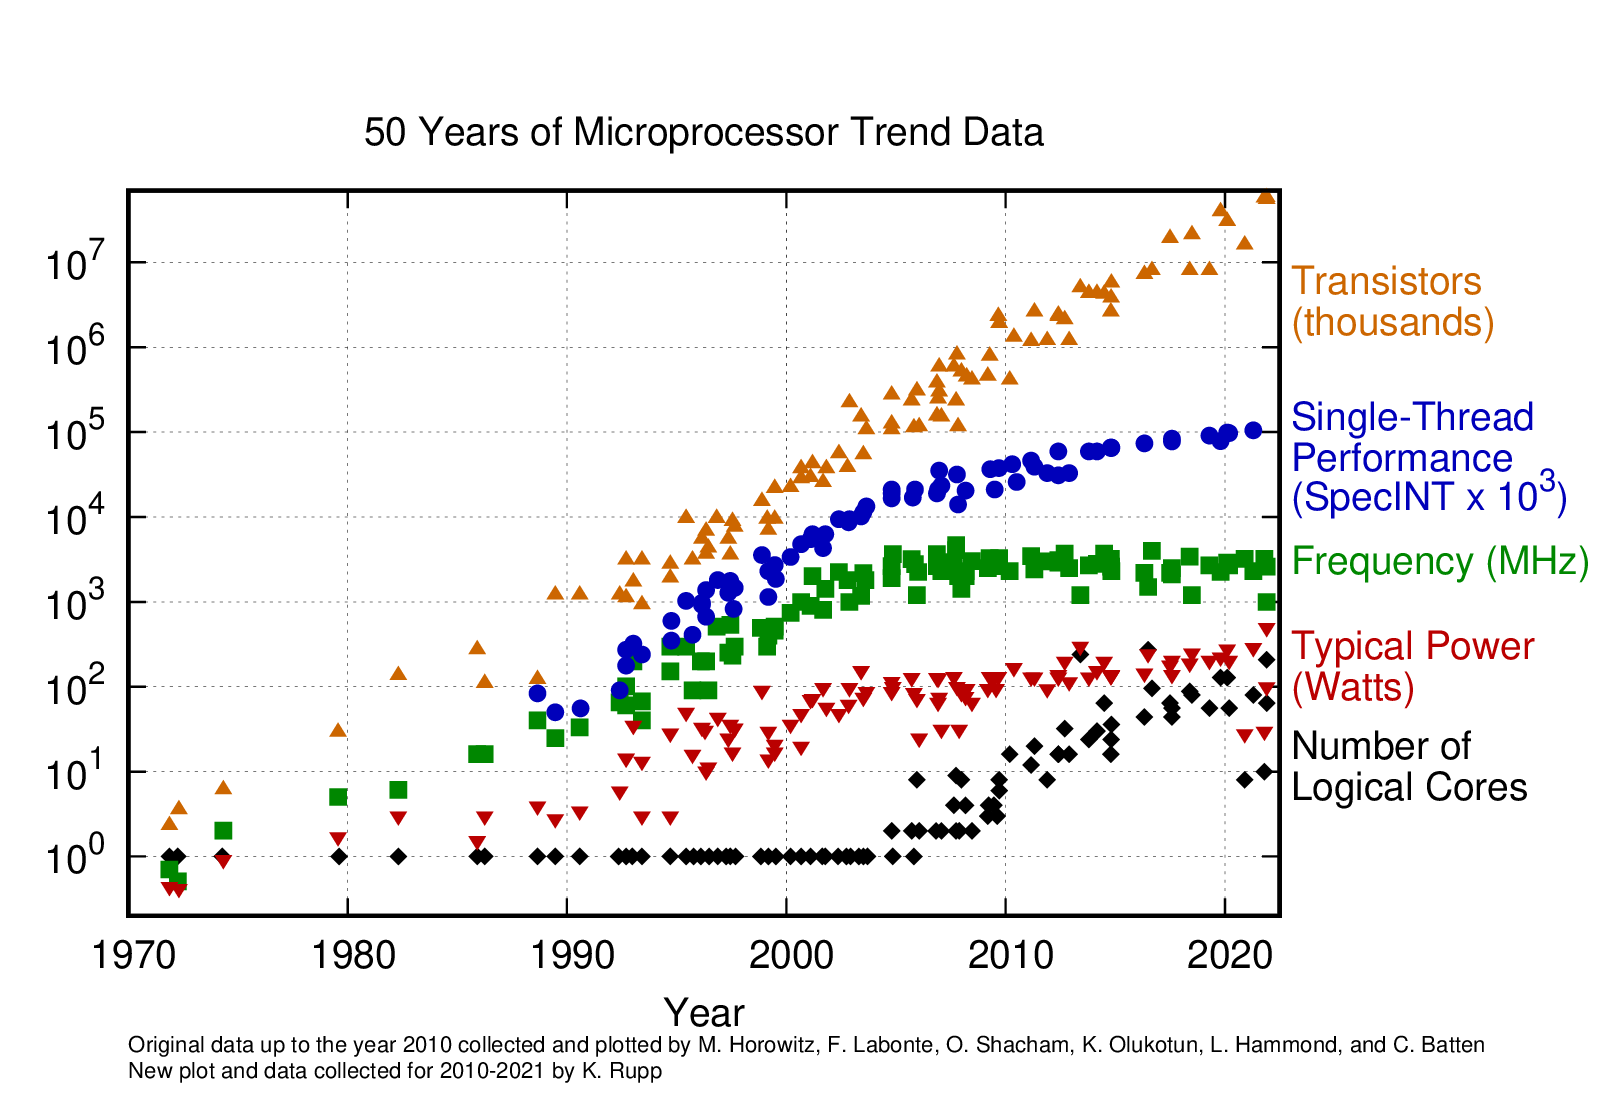
\includegraphics[width=\textwidth]{50-years-processor-trend.png}
    \caption{Evoluzione delle caratteristiche dei processori}
    \source{\url{https://github.com/karlrupp/microprocessor-trend-data}}
    \label{img:trend_proc}
\end{figure}

Al posto di aumentare il numero di transistor, negli ultimi due decenni sono state ideate nuove architetture che sfruttano il parallelismo: queste sono le architetture parallele, anche chiamate multicore o multiprocessore. Queste architetture sono sviluppate aggiungendo più processori fisici dentro ad un chip. Le prestazioni che si possono ottenere con le architetture parallele derivano quindi dalla suddivisione del lavoro che è distribuito in più unità operazionali.

Nella figura \ref{img:trend_proc} viene mostrata l'evoluzione dei processori nel corso degli ultimi decenni. In particolare, si può notare come la frequenza media dei processori si sia stabilizzata, mentre più o meno dalla metà degli anni 2000 sia cresciuto il numero di core logici, a seguito di ricerche sullo sviluppo delle architetture parallele.

\section{GPU e CUDA}

Esistono diverse tipologie di architetture parallele; in questa relazione ci interesseremo delle architetture basate su GPU. Queste architetture vengono chiamate GPGPU (General Purpose Graphics Processing Units), ovvero schede grafiche programmabili in maniera generica.

\begin{figure}[h]
    \centering
    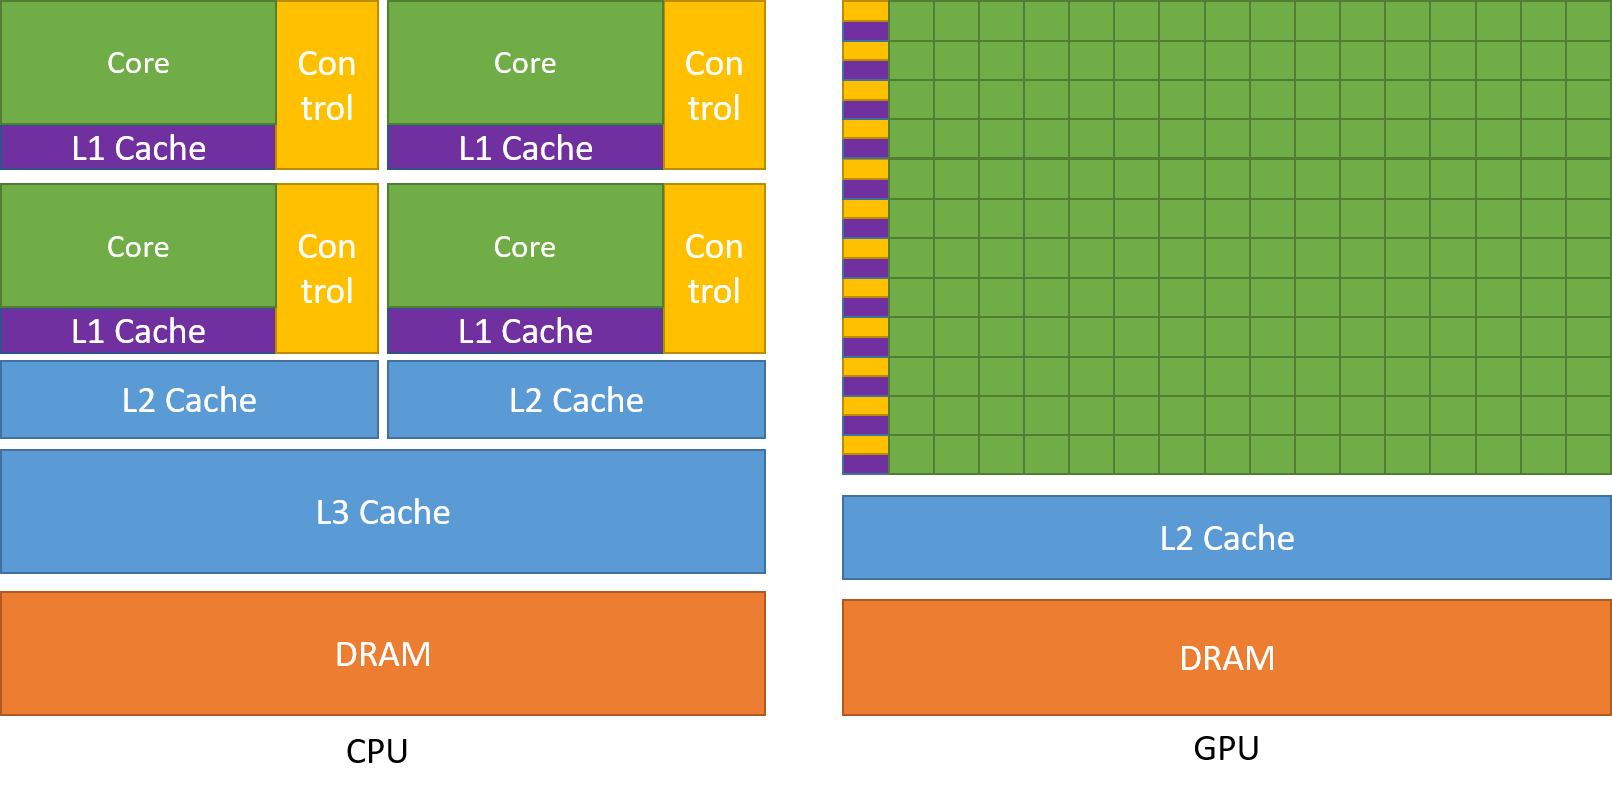
\includegraphics[width=\textwidth]{cpu-gpu-comparison.png}
    \caption[Confronto tra CPU e GPU]{Confronto tra l'architettura di una CPU e quella di una GPU. Da notare l'elevato numero di core della GPU.}
    \source{\url{https://docs.nvidia.com/cuda/cuda-c-programming-guide/index.html}}
    \label{img:cpu-gpu-comparison}
\end{figure}

Il nome di queste architetture potrebbe dare confusione dato che, in generale, la funzione di una scheda video è strettamente legata alla grafica. Il motivo per cui sono interessanti è per la presenza di un grande numero di core all'interno della scheda, molto più grande del numero di core presenti in una normale CPU (si tratta di due ordini di grandezza di differenza); questo implica che possono essere molto utili per programmi paralleli con dati di grandi dimensioni. La figura \ref{img:cpu-gpu-comparison} mostra le due architetture a confronto.

Le prime ricerche riguardanti la programmazione generale su GPU furono svolte nel 2001 e nel 2003; diventarono più popolari nel 2007 con l'avvento di CUDA.

CUDA (Compute Unified Device Architecture) è una piattaforma per il calcolo parallelo sviluppata da NVIDIA. Si tratta di una piattaforma che consente l'utilizzo delle schede grafiche NVIDIA per eseguire programmi paralleli, sfruttando appieno le loro potenzialità. La prima versione di CUDA è stata pubblicata nel 2007.

I concetti di base di CUDA sono molto semplici: CUDA prevede una separazione tra l'\textit{host}, che corrisponde la CPU, e il \textit{device}, che corrisponde ad una o più schede grafiche. Queste sono considerate unità indipendenti, che cooperano in modo asincrono: in particolare, l'\textit{host} ha la possibilità di invocare funzioni specifiche che vengono eseguite sul \textit{device}. Queste funzioni vengono dette \textit{kernel}; appena vengono chiamate, queste vengono eseguite in modo asincrono e restituiscono subito il controllo all'\textit{host}.

\subsection{Architettura di CUDA}

\begin{figure}[h]
    \centering
    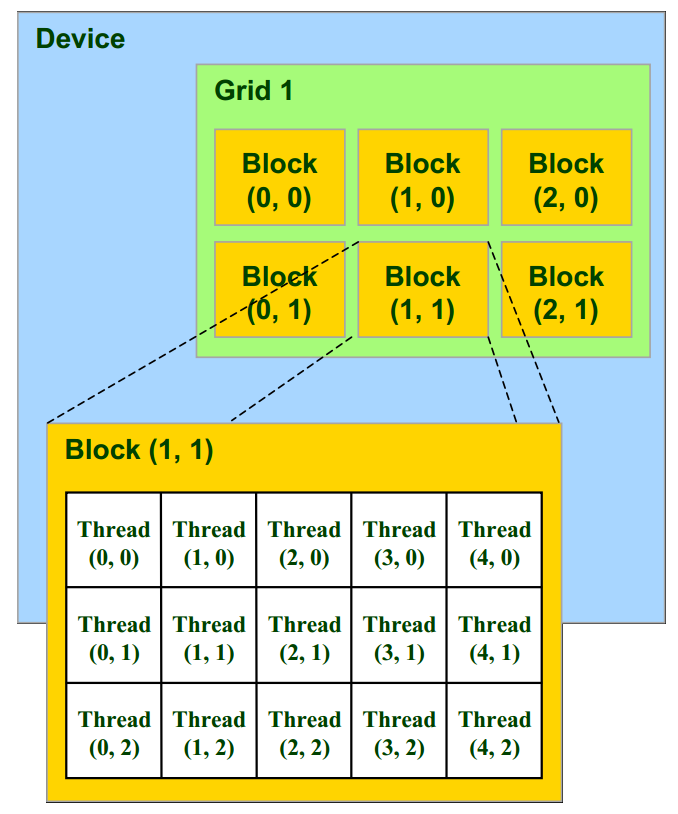
\includegraphics[width=6.5cm]{grids-and-blocks.png}
    \caption{Gerarchia dei thread in CUDA}
    \source{\url{https://ipython-books.github.io/58-writing-massively-parallel-code-for-nvidia-graphics-cards-gpus-with-cuda/}}
    \label{img:grids-and-blocks}
\end{figure}

In CUDA, l'unità minima di elaborazione è il \textbf{thread}. CUDA raggruppa logicamente i thread in più \textbf{blocchi}, e a loro volta i blocchi sono raggruppati in una \textbf{griglia} \cite{cudaguide}. La figura \ref{img:grids-and-blocks} mostra sinteticamente questa gerarchia.

Un blocco è considerato un unità indipendente di lavoro: esso può avere una, due o tre dimensioni, il che significa che può essere indicizzato in più dimensioni in base all'occorrenza; ogni blocco può essere eseguito in qualunque ordine all'interno di una griglia. Il numero di thread in un blocco è limitato a va fino a 1024 thread per blocco.

Una griglia rappresenta un lavoro affidato alla GPU: anch'esso può essere tridimensionale e non ha limiti sul numero di blocchi.

Lo \textbf{scheduling dei thread} in CUDA è completamente automatico: non è possibile scegliere quali e quanti core (che in CUDA vengono chiamati \textit{Streaming Multiprocessor}) debbano venire utilizzati.

\subsection{Struttura e gestione della memoria}

Quando si scrive un \textit{kernel}, non ci si deve mai preoccupare di come vengono gestiti i thread. Sarà l'hardware stesso a preoccuparsi, durante l'esecuzione, di effettuare lo scheduling migliore sfruttando al massimo l'hardware: in particolare, in CUDA esiste il concetto di \textit{warp}, che rappresenta l'unità minima di schedulazione e contiene un certo numero di thread (massimo 32). L'hardware raggruppa assieme in un \textit{warp} i thread che devono eseguire la stessa porzione di codice; i thread eseguono le istruzioni seguendo il paradigma SIMD.

Nel caso ci sia una biforcazione nel flusso di controllo (causato, ad esempio, da costrutti \verb|if-else|), la condizione viene calcolata per ogni thread, dopodichè vengono eseguiti i thread per cui è stata verificata, mentre gli altri rimangono fermi. L'hardware comunque può trasferire i thread che sono rimasti fermi in altri warp. La figura \ref{img:warp-branch} mostra un esempio visuale del problema.

\begin{figure}[h]
    \centering
    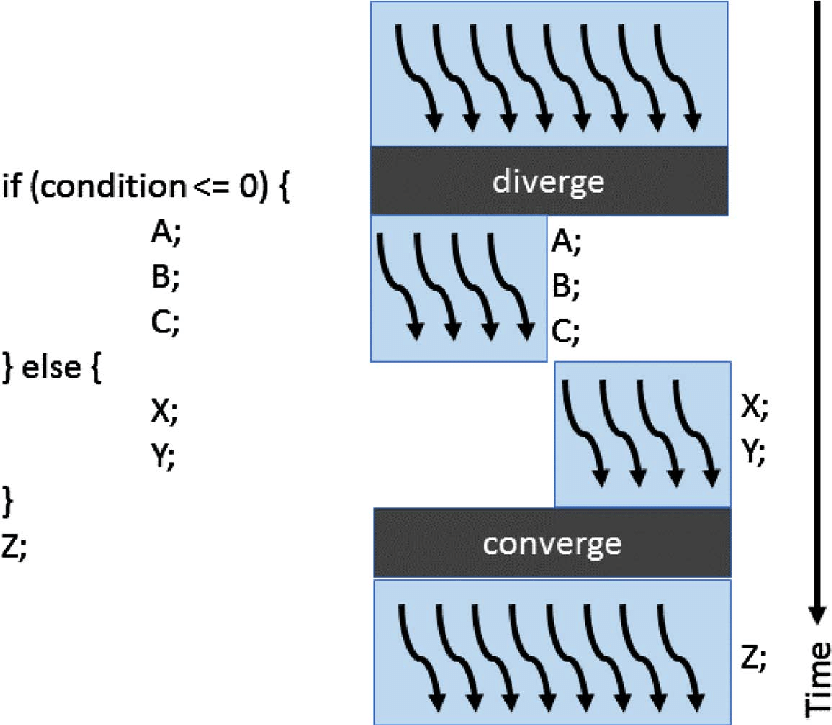
\includegraphics[width=6.5cm]{warp-branch.png}
    \caption{Esecuzione di un thread in caso di biforcazione}
    \source{\url{https://www.researchgate.net/figure/Warp-divergence-due-to-if-else-statements_fig15_317608134}}
    \label{img:warp-branch}
\end{figure}

La memoria in CUDA è suddivisa in più tipi:

\begin{itemize}
    \item \textbf{Memoria globale}: è la memoria più grande (alcuni GB). A questa memoria possono accedere ogni thread di ogni blocco, ma presenta una latenza di accesso più alta;
    \item \textbf{Memoria delle constanti}: una memoria persistente anch'essa accessibili da ogni thread, ma ci i thread possono accedere in sola lettura. L\'host può comunque accedere in scrittura. È più piccola, di soli 64 KB;
    \item \textbf{Memoria texture}: un'altra memoria di sola lettura e accessibile da tutti, ma è ottimizzata per le texture;
    \item \textbf{Memoria condivisa}: è una memoria molto veloce che viene condivisa tra tutti i thread di un solo blocco. Per blocco ci sono 48 KB di memoria condivisa;
    \item \textbf{Memoria locale}: una memoria dedicata per ogni thread, accessibile solo da esso. Non persiste tra l'esecuzione di due kernel;
\end{itemize}

La figura \ref{img:memory-hierarchy} mostra una rappresentazione visuale della memoria.

\begin{figure}[h]
    \centering
    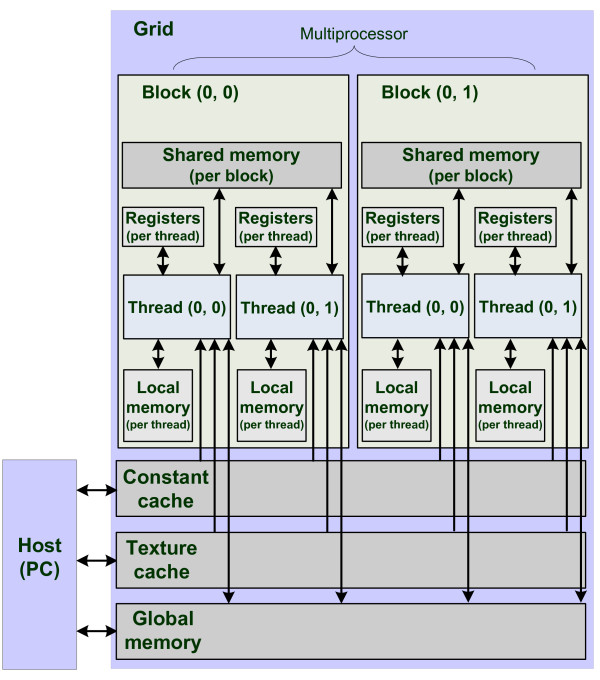
\includegraphics[width=8cm]{cuda-memory-hierarchy.jpg}
    \caption{La struttura della memoria in CUDA.}
    \source{\url{https://www.researchgate.net/figure/Memory-model-CUDA-memory-hierarchy_fig2_51529494}}
    \label{img:memory-hierarchy}
\end{figure}

In CUDA va prestata particolare attenzione all'accesso della memoria. Infatti, quando un thread esegue un accesso alla memoria anche molto piccolo (4 byte), la GPU legge almeno 32 byte consecutivi. Una caratteristica molto importante è il \textbf{raggruppamento degli accessi}: se più thread accedono a posizioni di memoria consecutive, la GPU raggruppa questi accessi in una sola lettura.

Questo in pratica significa che in CUDA il pattern di memorizzazione classico, ovvero l'Array-of-Structures, non è adeguato e si dovrebbe preferire la Structure-of-Arrays. Il primo consiste nel conversare i dati di un elemento (ad esempio un punto con coordinate x, y e z) in posizioni adiacenti di memoria: di conseguenza, un array di punti consisterà in un array di coordinate (x, y, z) che si ripete per ogni punto. Il secondo consiste nell'avere un array per ogni dato dell'elemento: si avrà un array per ogni coordinata X, coordinata Y e coordinata Z. La figura \ref{img:aos} mostra un confronto visuale dei due pattern.

Immaginiamo di avere più thread che devono leggere ognuno le coordinate X di ogni punto. Se i dati sono memorizzati mediante AoS, i valori in sè sarebbero più lontani tra loro, con la conseguenza di avere maggiori letture e maggior utilizzo del bus nel programma. Al contrario, con SoA si avrebbe tutti elementi adiacenti e si avrebbe bisogno di meno letture.

\begin{figure}
    \centering
    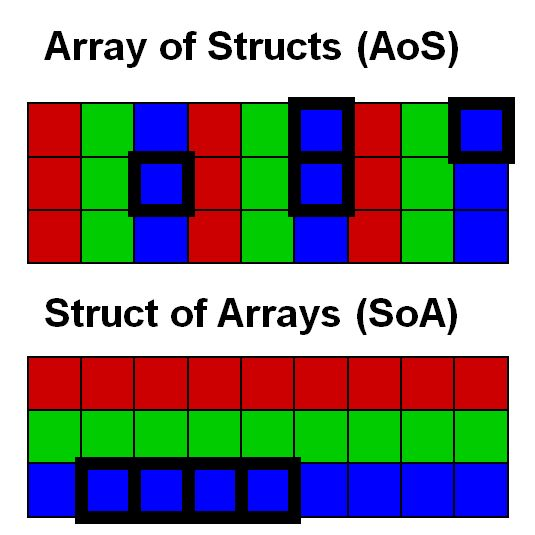
\includegraphics[width=5cm]{aos.jpg}
    \caption{AoS e SoA a confronto}
    \source{\url{https://asc.ziti.uni-heidelberg.de/en/node/18}}
    \label{img:aos}
\end{figure}

\subsection{Il linguaggio CUDA}

Per scrivere un kernel, CUDA prevede un apposito linguaggio: il linguaggio che si usa è un estensione del C e del C++ con l'aggiunta di parole chiave, funzioni di libreria ed altre caratteristiche per facilitare la scrittura del codice per GPU.

In particolare, CUDA aggiunge le seguenti parole chiave per le funzioni:

\begin{itemize}
    \item \verb|__host__|: usata per funzioni scritte per la CPU (presente di default se non ci sono altre parole chiave di CUDA);
    \item \verb|__device__|: usata per le funzioni scritte per la GPU e chiamate dalla GPU;
    \item \verb|__global__|: usata per le funzioni scritte per la GPU, ma chiamate dalla CPU. In essenza sono il punto d'entrata tra codice dell'\textit{host} e codice del \textit{device};
\end{itemize}

\verb|__host__| e \verb|__device__| possono essere combinati assieme. CUDA aggiunge anche le seguenti parole chiave per le variabili:

\begin{itemize}
    \item \verb|__constant__|: memorizza la variabile in memoria costante;
    \item \verb|__device__|: memorizza la variabile nella memoria globale della GPU. Essa è comunque accessibile dall'host tramite opportune funzioni;
    \item \verb|__shared__|: memorizza la variabile nella memoria shared. In questo caso, il suo accesso è limitato al singolo blocco;
\end{itemize}

L'estensione più importante in CUDA riguarda il modo in cui si chiamano le funzioni dichiarate \verb|__global__|: queste richiedono due parametri obbligatori, ovvero il numero di blocchi e il numero di thread per blocco da utilizzare per l'esecuzione.

\chapter{Stereo Vision}

La visione artificiale è il campo dell'informatica che si occupa di analizzare ed interpretare le immagini per ottenere un modello approssimato del mondo reale. In sostanza, si occupa di capire ed automatizzare compiti che il sistema di visione umano riesce a fare.

La Stereo Vision è una sottobranca della visione artificiale che si occupa di ottenere informazioni spaziali utilizzando due immagini (da qui viene il termine \textit{stereo}, che significa \textit{due}).

Gli uomini posseggono due occhi frontali che vedono il mondo esterno da due posizioni differenti: queste due posizioni vengono combinate, usando le piccole differenze presenti tra le due per recuperare le informazioni in 3D sull'ambiente esterno. L'idea di base della Stereo Vision è la simulazione di questo sistema: per far ciò si utilizzano due fotocamere, disposte orizzontalmente l'una all'altra, in modo che fungano come da occhi umani che guardano la scena di cui si è interessati. Le due immagini che si ottengono dalle fotocamere sono chiamate \textit{Stereo Pair}. La figura \ref{img:stereo_pair} ne mostra un esempio.

\begin{figure}[h]
    \centering
    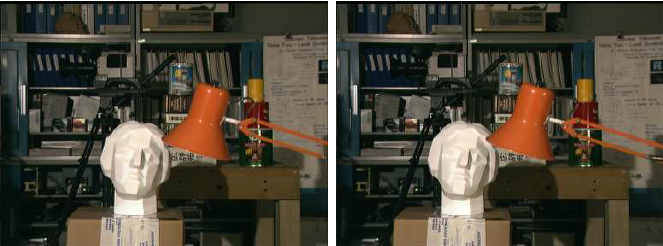
\includegraphics[width=\textwidth]{tsukuba-stereo-pair.png}
    \caption[Un esempio di \textit{stereo pair}.]{Uno \textit{stereo pair}. La seconda immagine è leggermente spostata orizzontalmente rispetto alla prima.}
    \source{\url{https://www.researchgate.net/figure/Tsukuba-stereo-pair_fig1_278622997}}
    \label{img:stereo_pair}
\end{figure}

Un problema importante nella Stereo Vision è come inferire la profondità degli oggetti della scena usando le due immagini prese dalle fotocamere \cite{imagevideohandbook}. È qui che entrano in gioco gli algoritmi di \textit{Stereo Matching}: durante la fase di analisi delle due immagini, si cerca una corrispondenza (\textit{match}) tra un oggetto di un immagine e la posizione dell'oggetto nell'altra immagine: la differenza della sua posizione nelle due immagini determina la posizione finale dell'oggetto. Le informazioni che si ottengono sulla profondità degli oggetti vengono chiamate nel loro complesso \textit{mappa di disparità}. Una mappa di disparità si può vedere nella figura \ref{img:disparity_map}.

\begin{figure}[h]
    \centering
    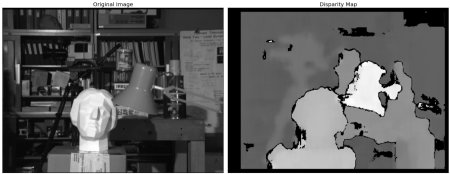
\includegraphics[width=\textwidth]{disparity_map.jpg}
    \caption[Esempio di mappa di disparità.]{Esempio di mappa di disparità. Le regioni più chiare indicano oggetti più vicini, mentre quelle più scure indicano oggetti più lontani.}
    \source{\url{https://docs.opencv.org/4.x/dd/d53/tutorial_py_depthmap.html}}
    \label{img:disparity_map}
\end{figure}

\section{Le fasi di analisi delle immagini}

Per estrarre le informazioni 3D, la maggior parte degli algoritmi di Stereo Vision seguono i seguenti passi:

\begin{enumerate}
    \item Nel caso le immagini siano distorte o abbiano qualche difetto, bisognerà effettuare una \textbf{calibrazione della fotocamera}.
    \item Le immagini vengono riproiettate in un piano comune per permettere il confronto diretto. Questo passo viene detto \textbf{rettificazione delle immagini} e in generale si effettua soltanto se i piani delle due fotocamere non giacciono sulla stessa linea (questa linea viene chiamata \textit{baseline}.
    \item Si fa il \textbf{matching} tra le due immagini e si crea la mappa di disparità. Questo di solito avviene pixel per pixel: dato il pixel $p_{1}$ della prima immagine, si cerca un secondo pixel $p_{2}$ nella seconda immagine che corrisponda al primo. Come calcolare se due pixel corrispondono dipende dall'algoritmo.
    \item Opzionalmente, si effettua una \textbf{ricostruzione} in 3D della scena. Questo viene fatto determinando le coordinate 3D di ogni punto a partire dalle coordinate 2D delle coppie di punti corrispondenti nelle immagini.
\end{enumerate}

\section{Tecniche di \textit{matching}}

L'approccio classico per lo stereo matching è: per ogni pixel $p = (x, y)$ nell'immagine di partenza, si trova la linea corrispondente nell'immagine di destinazione, poi si trova il pixel $p'$ più somigliante nella linea. Nei casi più semplici, la linea corrispondente è la coordinata $y$ del punto $p$.

Il calcolo della \textbf{somiglianza} differisce in ogni algoritmo, ma in generale viene calcolata utilizzando la regione intorno al punto. Si definiscono due \textit{finestre} di grandezza $N \times N$: $W (x, y)$, centrata nel punto $p$, e $W'$, che viene fatta scorrere in orizzontale lungo la linea. Ad ogni scorrimento corrisponde un nuovo punto $p'$. Per ogni punto $p'$ trovato, si calcola una metrica particolare derivata dall'intorno. Tre metriche popolari sono la \textit{Correlazione Normalizzata}, la \textit{Sum of Squared Differences} e la \textit{Sum of Absolute Differences} \cite{stereomatchingalgos}.

Un approccio alternativo consiste nell'\textit{edge matching} (\textit{corrispondenza dei contorni}). In questo caso per le due immagini si trovano i contorni, poi si fa il \textit{match} dei contorni in modo simile al metodo delle finestre: in questo caso si calcola la somiglianza tra contorni. La figura \ref{img:contours} mostra un immagine di cui sono stati prelevati i contorni.

\begin{figure}[h]
    \centering
    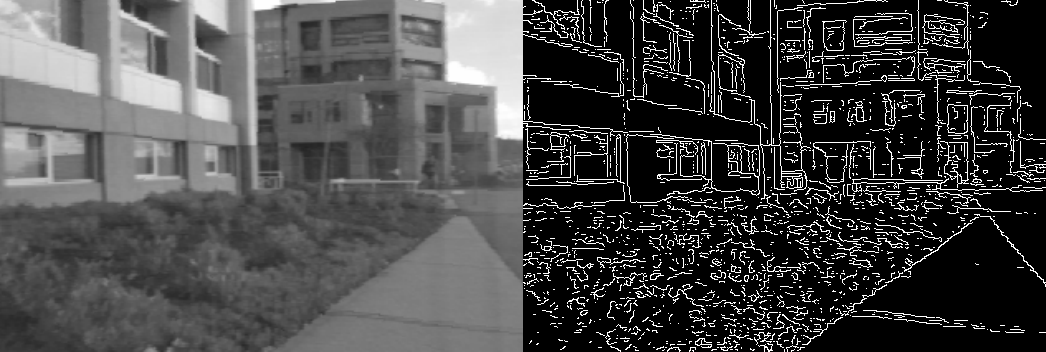
\includegraphics[width=\textwidth]{contours.png}
    \caption{I contorni di un immagine.}
    \label{img:contours}
\end{figure}



\chapter{La \textit{Connection Machine} e *Lisp}

L'algoritmo di stereo matching che presentiamo fu descritto e implementato per la \textbf{Connection Machine CM-2} nel linguaggio \textbf{*Lisp}. In questo capitolo diamo una breve descrizione delle loro caratteristiche, in modo da poter confrontare l'algoritmo originale con la versione in CUDA.

\section{La Connection Machine CM-2}

\begin{figure}[h]
    \centering
    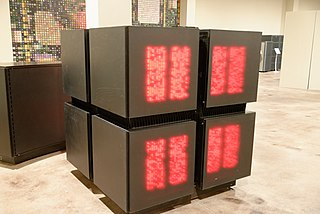
\includegraphics[width=7cm]{connection-machine.jpg}
    \caption{Il design esterno della Connection Machine CM-2.}
    \source{\url{https://commons.wikimedia.org/wiki/File:Computer_Museum_of_America_(51).jpg}}
    \label{img:connection_machine}
\end{figure}

La \textit{Connection Machine CM-2} fa parte di una serie di supercomputer sviluppati dall'azienda Thinking Machines nei primo anni 80. La macchina era un supercomputer parallelo basata sul parallelismo a livello di dati (\textit{data level parallelism}), che consiste nell'eseguire un'operazione su più dati in parallelo, in contrasto con il parallelismo a livello di istruzioni, che consiste nell'eseguire in parallelo le istruzioni che possono essere eseguite indipendentemente \cite{originalalgo}. In pratica, ciò significa che la Connection Machine operava come una gigantesca macchina SIMD (Single Instruction Multiple Data). La figura \ref{img:connection_machine} ne mostra una foto dall'esterno.

La macchina, per eseguire i programma, utilizzava una parte di front-end, dove veniva memorizzato il programma e dove veniva eseguito il codice seriale. Quando un programma incontrava istruzioni parallele (istruzioni che operava sui dati in modo parallelo), le passava all'hardware della Connection Machine: questo era composto da 65535 processori, ognuno con 4096 bit di memoria.

Ogni processore operava su un solo elemento: se c'erano meno di 65535 elementi, allora i processori rimanenti venivano disabilitati; se ce n'erano di più, allora la macchina operava con processori virtuali. I processori potevano comunicare tra di loro attraverso un sistema di inter-connessione chiamato \textit{router}: questo funzionava con meccanismi di comunicazione a scambio di messaggi ed era implementato in software.

\section{*Lisp}

Lisp è un linguaggio di programmazione ideato all'inizio degli anni 60 da John McCarthy. Si tratta di un linguaggio basato sui paradigmi imperativo e funzionale, con una sintassi molto unica. Il seguente codice presenta un esempio del linguaggio; si tratta di una funzione che trova se un elemento esiste in un array:

\newpage

\begin{lstlisting}[caption={Esempio di codice Lisp. Questa funzione implementa la ricerca nell'array in maniera ricorsiva, in concordanza con il paradigma funzionale.}]
(defun contains-element (arr i element)
  (if (= i (array-dimension arr 0))
    0
    (if (= (aref arr i) element)
      1
      (contains-element arr (+ i 1) element))))
\end{lstlisting}

Il Lisp ha molti dialetti e *Lisp è uno di questi (in particolare, è un dialetto del Common Lisp). *Lisp, come linguaggio pensato per essere usato nella Connection Machine, aggiunge nuove caratteristiche per la programmazione parallela: ad esempio, molti costrutti come \verb|if| e \verb|=| hanno una versione parallela che agiscono su tutti i dati in contemporanea. In particolare, introduce una struttura dati, la \textit{pvar}, che rappresenta una collezione di valori memorizzati uno per ogni processore \cite{starlisp}. Il seguente codice mostra un esempio di codice *Lisp, che è una traduzione della funzione sopra:

\begin{lstlisting}[caption={Esempio di codice *Lisp. Questa versione della funzione implementa la ricerca in parallelo su tutti gli elementi dell'array.}]
(*defun contains-element (pvar element)
  (if!! (=!! pvar element)
        (!! 1)
        (!! 0)))
\end{lstlisting}

\chapter{Descrizione dell'algoritmo di \textit{stereo matching}}

L'algoritmo di \textit{stereo matching} che andiamo a presentare ha come obbiettivo il disegnare le linee di livello di un'area geografica. Questo problema viene chiamato \textit{contour mapping} e consiste nell'estrarre informazioni sull'altezza da immagini che memorizzano informazioni sulla luminosità dell'area. L'immagine risultante viene chiamata \textit{contour map} (mappa dei contorni o dei livelli).

L'algoritmo prende come input due immagini aeree di un'area geografica: le due immagini devono essere uno \textit{stereo pair} e devono essere siano in bianco e nero, ovvero all'inizio dell'algoritmo le due immagini devono rappresentare la luminosità che c'è in ogni punto dell'area geografica.

L'algoritmo è composto da tre fasi:

\begin{enumerate}
    \item La ricerca dei bordi o contorni;
    \item La ricerca di corrispondenze tra i contorni trovati;
    \item Il disegno delle linee di livello;
\end{enumerate}

Questo algoritmo si tratta di un algoritmo di \textit{edge matching}: le operazioni più importanti sono quelle legate alla ricerca e alla corrispondenza dei bordi (\textit{edges}).

Per avere più dettagli sull'implementazione originale dell'algoritmo, si può consultare \cite{originalalgo}.

\section{Ricerca ed estrazione dei bordi}

La ricerca dei contorni avviene indipendentemente su tutte e due le immagini. L'algoritmo definisce un contorno come una linea che giace sul confine tra aree di luminosità molto diversa. A questo proposito, l'algoritmo da una classificazione per ogni pixel basandosi sui suoi intorni: se da un lato del pixel la luminosità è molto differente che dall'altro, allora il pixel viene classificato come un pixel del contorno. Questa operazione è un esempio di \textit{local neighborhood operation}, operazione locale sui vicini.

La seguente funzione in *Lisp mostra l'implementazione originale dell'operazione. Questa funzione si occupa solo di un pixel: prima calcola la media della luminosità nei lati destro e sinistro del pixel, poi calcola la differenza di luminosità e la confronta con una certa soglia: se questa risulta maggiore, allora il pixel viene considerato come parte di un bordo.

A riga 19, la soglia è moltiplicata con la media complessiva di luminosità: in questo modo, la soglia si adatta all'immagine, diventando minore o maggiore a seconda di quanto sia ``luminosa'' l'immagine in quel punto.

\begin{lstlisting}[style=mystyle]
(*defun find-edges-between-left-and-right!! (brightness-pvar threshold)
  (*let*
    ((average-brightness-on-the-left
       (/!! (+!! (pref-grid-relative!! brightness-pvar (!! -1) (!! -1))
                 (pref-grid-relative!! brightness-pvar (!! -1) (!!  0))
                 (pref-grid-relative!! brightness-pvar (!! -1) (!!  1)))
            (!! 3.0)))
     (average-brightness-on-the-right
       (/!! (+!! (pref-grid-relative!! brightness-pvar (!!  1) (!! -1))
                 (pref-grid-relative!! brightness-pvar (!!  1) (!!  0))
                 (pref-grid-relative!! brightness-pvar (!!  1) (!!  1)))
            (!! 3.0)))
     (average-brightness-overall
       (/!! (+!! average-brightness-on-the-left
                 average-brightness-on-the-right)
            (!! 2.0))))
    (if!! (>!! (absolute-value!! (-!! average-brightness-on-the-left
                                      average-brightness-on-the-right))
               (*!! (!! threshold) average-brightness-overall))
          (!! 1)
          (!! 0))))
\end{lstlisting}

Questa e altre funzioni simili, che confronteranno anche gli altri lati (sopra, sotto e nelle diagonali), vengono combinate con la seguente funzione, per garantire il ritrovo di ogni contorno:

\begin{lstlisting}[style=mystyle]
(*defun find-all-edges!! (brightness-pvar threshold)
  (if!! (or!! (=! (!! 1) (find-edges-between-left-and-right!!
                           brightness-pvar threshold))
              (=! (!! 1) (find-edges-between-above-and-below!!
                           brightness-pvar threshold))
              (=! (!! 1) (find-edges-between-upper-left-and-lower-right!!
                           brightness-pvar threshold))
              (=! (!! 1) (find-edges-between-lower-left-and-upper-right!!
                           brightness-pvar threshold)))
        (!! 1)
        (!! 0)))
\end{lstlisting}

Il risultato è una nuova immagine con solo valori 0 o 1, dove gli uni indicano i bordi.

\section{Ricerca di corrispondenze tra i bordi}

Il prossimo passo consiste nell'\textit{edge matching} tra le immagini dei bordi ottenute. Questo passo viene fatto con un processo di scorrimento: la prima immagine resta ferma, mentre la seconda viene fatta scorrere sulla prima. Per ogni scorrimento (\textit{shift}), tutti i pixel della prima immagine vengono confrontati con la seconda: se un pixel della prima è uguale al pixel alla stessa posizione nella seconda, allora si ha una corrispondenza. Il risultato è un immagine binaria dove gli uni indicano corrispondenze.

La funzione seguente è l'implementazione originale. L'array alla riga 1 memorizza le immagini risultanti per ogni scorrimento. L'operazione alla riga 6 implementa l'operazione di scorrimento: la funzione \verb|pref-grid-relative| esegue un operazione di indicizzazione relativa, ovvero prende un immagine in input, la sposta di \verb|i| posizioni in orizzontale e ritorna una nuova immagine. Il risultato è che ad ogni ciclo di \verb|dotimes| (che corrisponde ad un ciclo \verb|for| da 0 a 30), l'immagine destra sarà spostata orizzontalmente e confrontata con l'immagine di sinistra.

\begin{lstlisting}[style=mystyle]
(defvar *array-of-pvars-holding-matches-at-each-shift* (make-array 30))

(*defun fillup-pvars-wherever-edges-align (left-edges right-edges)
  (dotimes (i 30)
    (aset (if!! (=!! left-edges
                     (pref-grid-relative!! right-edges (!! i) (!! 0))
                     )      ; ^ this PREF-GRID-RELATIVE!! accomplishes
                (!! 1)      ; the "sliding" process.
                (!! 0))
          *array-of-pvars-holding-matches-at-each-shift*
          i)))
\end{lstlisting}

A questo punto, l'algoritmo usa le informazioni appena calcolate per misurare la qualità dell'allineamento: per ogni pixel, si calcola quale scorrimento è il migliore tra tutti. L'indice dello scorrimento migliore corrisponderà direttamente all'altezza di quel pixel.

Lo scorrimento migliore viene calcolato in più fasi: prima, per ogni scorrimento si assegna un punteggio, che indicherà la qualità di quello scorrimento per quel pixel. Il punteggio per ogni pixel viene calcolato con un'altra operazione locale sui vicini: vengono contati il numero di pixel nell'intorno che hanno avuto una corrispondenza in quello scorrimento. Nell'implementazione originale, questo intorno è un quadrato di lato variabile (di solito 21) e vengono sommati tutti i pixel posti a 1 in precedenza.

La funzione seguente esegue l'operazione descritta in parallelo per ogni pixel di un immagine.

\begin{lstlisting}[style=mystyle]
(*defun add-up-all-pixels-in-a-square (pvar width-of-square)
  (let ((one-half-the-square-width (/ width-of-square 2)))
    (*let ((total (!! 0)))
      (dotimes (relative-x width-of-square)
        (dotimes (relative-y width-of-square)
          (*set total
                (+!! total
                     (pred-grid-relative!!
                       pvar
                       (- relative-x one-half-the-square-width)
                       (- relative-y one-half-the-square-width))))))
      total)))
\end{lstlisting}

Per calcolare i punteggi per ogni scorrimento, basta usare la funzione precedente in un ciclo. La funzione seguente implementa questo ciclo, poi esclude dal calcolo della qualità tutti i pixel che non fanno parte dei bordi (per questi il punteggio è zero).

\begin{lstlisting}[style=mystyle]
(defvar *array-of-pvars-holding-scores-at-each-shift* (make-array 30))

(*defun fillup-pvars-with-match-scores (width-of-square)
  (dotimes (i 30)
    (*let ((sum-of-all-nearby-pixels
            (add-up-all-pixels-in-a-square
              (aref *array-of-pvars-holding-matches-at-each-shift* i)
              width-of-square)))
      (*if (=!! (aref *array-of-pvars-holding-matches-at-each-shift* i)
                (!! 1)) ;;; record a score wherever there was a match-up
           (*set sum-of-all-nearby-pixels
                 *array-of-pvars-holding-scores-at-each-shift*
                 i)))))
\end{lstlisting}

Infine, per trovare il migliore scorrimento per ogni pixel, basta usare la classica operazione di ricerca del massimo. La funzione seguente implementa prima un ciclo che trova i punteggi massimi (righe 6-10), poi trova a quali scorrimenti sono associati quei punteggi (righe 13-16). Il risultato della funzione è un immagine con gli indici degli scorrimenti migliori, che corrispondono all'altezza per ogni pixel.

\begin{lstlisting}[style=mystyle]
(*defun find-the-shifts-of-the-highest-scoring-matches ()
  (*let ((best-scores (!! 0))
        (winning-shifts (!! 0)))
    ;; the following DOTIMES loop makes sure that each pixel in the
    ;; BEST-SCORES pvar contains the maximum score found at any shift.
    (dotimes (i 30)
      (*if (>!! (aref *array-of-pvars-holding-scores-at-each-shift* i)
                best-scores)
           (*set best-scores
                 (aref *array-of-pvars-holding-scores-at-each-shift* i))))
    ;; the following DOTIMES loop records a "winning" shift at every
    ;; pixel whose score is the best.
    (dotimes (i 30)
      (*if (=!! (aref *array-of-pvars-holding-scores-at-each-shift* i)
                best-scores)
           (*set winning-shifts (!! (1+ i)))))
    winning-shifts))
\end{lstlisting}

\section{Disegno delle linee di livello}

Il processo fatto finora ci dà un'immagine che rappresenta l'altezza dell'area ad ogni pixel. Le altezze memorizzate però valgono solo per i pixel che giacciono sui bordi: essenzialmente tra i bordi ci sono ancora dei buchi e serve un altro passo per trovare le informazioni mancanti per questi buchi. L'algoritmo trova queste informazioni usando un operazione di interpolazione: per ogni pixel la cui altezza è zero, calcola una media sugli intorni dei pixel.

Compiendo questa operazione una sola volta, solo i pixel giacenti vicino ai bordi si riempirebbero, dato che per un pixel ad altezza 0 a sua volta circondato da pixel ad altezza 0 la media rimane 0. Per questo l'operazione viene ripetuta un certo numero di volte, riempiendo gradualmente i buchi ad ogni iterazione, finché tutti i pixel diventino coperti e nessuno abbia altezza 0.

\begin{lstlisting}[style=mystyle]
(defun fill-in-web-holes (web-of-known-elevations times-to-repeat)
  (dotimes (i times-to-repeat)
    (*let ((not-fixed (zerop!! web-of-known-elevations)))
      (*if not-fixed
        (*set web-of-known-elevations
              (/! (+!!
                    (pref-grid-relative!!  web-of-known-elevations
                      (!!  1) (!!  0))  ; neighbor to the right
                    (pref-grid-relative!!  web-of-known-elevations
                      (!!  0) (!!  1))  ; neighbor above
                    (pref-grid-relative!!  web-of-known-elevations
                      (!! -1) (!!  0))  ; neighbor to the left
                    (pref-grid-relative!!  web-of-known-elevations
                      (!!  0) (!! -1))) ; neighbot below
                  (!! 4))))))
  ;;; this is now a more or less smooth surface.
  web-of-known-elevations)
\end{lstlisting}

L'ultimo passo consiste nel disegnare le linee di livello. L'implementazione originale prende in input il numero di linee da tracciare, divide le altezze in più intervalli e traccia una linea per ogni intervallo. La variabile \verb|contour-line-interval| a riga 9 rappresenta quante ``altezze'' si deve saltare prima di tracciare una nuova linea.

\begin{lstlisting}[style=mystyle]
(defun draw-contour-map (number-of-contour-lines
                         pvar-of-smooth-continuous-elevations)
  ;; The idea is to divide the whole range of elevations into
  ;; a number of intervals, then to draw a contour line at every
  ;; interval.
  (let ((max-elevation (*max pvar-of-smooth-continuous-elevations))
        (min-elevation (*min pvar-of-smooth-continuous-elevations))
        (range-of-elevations (- max-elevation min-elevation))
        (contour-line-interval (/ range-of-elevations
                                  number-of-contour-lines)))
    ;; Now the variable CONTOUR-LINE-INTERVAL tells us how many
    ;; elevations, or shifts, to skip between contour lines.
    (if!! (zerop!!
            (mod!! (-!! pvar-of-smooth-continuous-elevations
                        (!! min-elevation))
                          (!! contour-line-interval)))
          (!! 1)        ;; this if!! draws all the elevation contours
          (!! 0))))     ;; at once, returning a bit map suitable
                        ;; for immediate display.
\end{lstlisting}

\chapter{Progettazione e traduzione}

Basandoci sulla descrizione dell'algoritmo nel capitolo precedente, ne presentiamo una traduzione in CUDA. Il codice nel suo complesso è reperibile al link \cite{thecode}.

\section{Ricerca ed estrazione dei bordi}

La prima funzione tradotta è stata quella che implementa la classificazione di un pixel come parte del bordo. Un numero pari a \verb|width * height| di thread eseguono la funzione in parallelo: ogni thread è identificato da una coppia di coordinate \verb|x| e \verb|y|.

\begin{lstlisting}[style=mystyle]
__device__ int find_edges_left_right(double *brightness,
        int width, int height, int x, int y, double threshold)
{
    double avg_left  = (brightness[idx(x-1, y-1, width, height)]
                     +  brightness[idx(x-1, y  , width, height)]
                     +  brightness[idx(x-1, y+1, width, height)]) / 3.0;
    double avg_right = (brightness[idx(x+1, y-1, width, height)]
                     +  brightness[idx(x+1, y  , width, height)]
                     +  brightness[idx(x+1, y+1, width, height)]) / 3.0;
    double overall   = (avg_left + avg_right) / 2.0;
    return fabs(avg_left - avg_right) > CLAMP(threshold * overall,
                                                0.0, 1.0);
}
\end{lstlisting}

Da questa funzione notiamo alcuni dettagli:

\begin{itemize}
    \item La descrizione originale dell'algoritmo non dice niente sui tipi di dati: si sa solo che le immagini in input sono in bianco e nero, ovvero in scala di grigi, ma non dice nulla sul range di valori. La rappresentazione più comune per immagini in scala di grigi è avere un valore da 0 a 255 per ogni pixel; in questo programma, però, si è scelto un'altra rappresentazione: i valori sono in virgola mobile (\verb|double|) e vanno da 0 a 1, dove 0 indica il nero e 1 indica il bianco. Si è scelto questo per via del fatto che l'operazione di moltiplicazione della soglia a riga 11 ha senso solo con questa rappresentazione (anche la soglia ha un valore da 0 a 1).
    \item Mentre in *Lisp le funzioni parallele agiscono su tutti gli elementi in automatico, in CUDA non è così: bisogna sempre fare un indicizzazione esplicita all'accesso degli array.
    \item Il codice in *Lisp non ha nessun controllo sui bordi della \textit{pvar}: è il linguaggio stesso che fa questi controlli. CUDA non fa nessun controllo, per cui si è scelto che la funzione \verb|idx|, che ha il compito di semplificare l'indicizzazione, faccia un \textit{wrap-around} ogni volta che gli indici sono superiori ai bordi (\verb|w| e \verb|h|).
    \item Infine, la funzione \verb|CLAMP| fa si che il risultato della moltiplicazione resti tra 0 e 1.
\end{itemize}

Come nell'implementazione originale, questa funzione viene implementata per tutti gli altri lati e le quattro funzioni risultanti vengono combinate:

\newpage

\begin{lstlisting}[style=mystyle]
__global__ void find_all_edges(double *brightness, int w, int h,
        double threshold, u8 *edges)
{
    DECLARE_INDEXES(w, h)
    edges[IDX(x, y, w)] =
              find_edges_left_right(brightness, w, h, x, y, threshold)
     ||       find_edges_top_bottom(brightness, w, h, x, y, threshold)
     || find_edges_upleft_downright(brightness, w, h, x, y, threshold)
     || find_edges_downleft_upright(brightness, w, h, x, y, threshold);
}
\end{lstlisting}

Il risultato viene messo in \verb|edges|. Quest'ultimo è un immagine \textit{binaria}, ovvero un immagine con solo 0 o 1, dove 0 questa volta indica il bianco e 1 il nero.

La macro \verb|DECLARE_INDEXES| dichiara una coppia di coordinate \verb|x| e \verb|y| che identifica il thread che sta eseguendo, poi fa un controllo su quest'ultima per sapere se attivare il thread per questo kernel. Questo controllo serve nel caso vengano usati troppi thread (che può capitare se la larghezza o l'altezza delle immagini di input non sono multipli della dimensione del blocco predefinita). La macro viene usata in ogni kernel e viene espansa nel seguente codice:

\begin{lstlisting}
int x = threadIdx.x + blockIdx.x * blockDim.x;
int y = threadIdx.y + blockIdx.y * blockDim.y;
if (x >= width || y >= height)
    return;
\end{lstlisting}

La funzione \verb|IDX|, utilizzata per indicizzare \verb|edges|, è una versione di \verb|idx| che non fa nessun \textit{wrap-around}, dato che in questo caso è impossibile che \verb|x| e \verb|y| siano fuori dai bordi.

\section{Ricerca di corrispondenze tra i bordi}

La creazione di strutture dati in CUDA non è trasparente come in *Lisp: per molte strutture si richiede l'allocazione esplicita. Le seguenti funzioni mostrano come viene gestito l'array \verb|matches|, che ha il compito di memorizzare, per ogni scorrimento, il risultato dell'\textit{edge matching}.

\begin{lstlisting}[style=mystyle]
__device__ u8 *matches[NUM_SHIFTS];

void allocate_matches(int width, int height)
{
    u8 *tmp[NUM_SHIFTS];
    for (int i = 0; i < NUM_SHIFTS; i++)
        tmp[i] = ALLOCATE_GPU(u8, width * height);
    cudaMemcpyToSymbol(matches, tmp, sizeof(tmp));
}

void free_matches()
{
    u8 *tmp[NUM_SHIFTS];
    cudaMemcpyFromSymbol(tmp, matches, sizeof(tmp));
    for (int i = 0; i < NUM_SHIFTS; i++)
        cudaFree(tmp[i]);
}
\end{lstlisting}

La funzione \verb|ALLOCATE_GPU| è un semplice \textit{wrapper} della funzione \verb|cudaMalloc| che ne semplifica il funzionamento. Dato che l'\textit{host} non ha accesso diretto alla memoria sul \textit{device}, si usa la funzione \verb|cudaMemcpyToSymbol| per aggiornare \verb|matches|.

La funzione seguente è una traduzione diretta della funzione originale \verb|fillup-pvars-wherever-edges-align|. Da notare che gli elementi di \verb|matches| sono tutte immagini binarie.

\begin{lstlisting}[style=mystyle]
__global__ void fillup_matches(u8 *left_edges, u8 *right_edges,
        int width, int height)
{
    DECLARE_INDEXES(width, height)
    int index = IDX(x, y, width);
    for (int i = 0; i < NUM_SHIFTS; i++) {
        int shift = idx(x+i, y, width, height);
        // ^ the +i accomplishes the sliding process
        matches[i][index] = left_edges[index] == right_edges[shift];
    }
}
\end{lstlisting}

La seguente porzione di codice mostra la traduzione della funzione \\ \verb|add-up-all-pixels-in-a-square|. Il doppio ciclo \verb|for| è leggermente differente dalla versione originale, dato che inizia da \verb|-half| e arriva a \verb|+half|.

\begin{lstlisting}[style=mystyle]
__global__ void addup_pixels_in_square(int i, int width, int height,
        int square_width, i32 *total)
{
    DECLARE_INDEXES(width, height)
    u8 *pixels = matches[i];
    int cur = IDX(x, y, width);
    int half = square_width / 2;
    for (int sy = -half; sy <= half; sy++) {
        for (int sx = -half; sx <= half; sx++) {
            int rel = idx(x + sx, y + sy, width, height);
            total[cur] += (i32) pixels[rel];
        }
    }
}
\end{lstlisting}

Per calcolare i punteggi ci serviamo di una struttura dati simile a \verb|matches|: le funzioni per allocare e liberare la memoria sono equivalenti.

Le seguenti funzioni corrispondono alla funzione originale \\ \verb|fillup-pvars-with-match-scores|, ma sono divise in due per via della \verb|cudaMemset| fatta prima di riempire l'array \verb|sum|: quest'ultimo viene usato in questo modo per evitare di fare più allocazioni.

\begin{lstlisting}[style=mystyle]
__device__ i32 *scores[NUM_SHIFTS];

/* ... functions for managing scores omitted ... */

__global__ void record_score(int i, i32 *sum, int width, int height)
{
    DECLARE_INDEXES(width, height)
    int index = IDX(x, y, width);
    // record a score whenever there was a match-up
    if (matches[i][index] == 1)
        scores[i][index] = sum[index];
}

void fillup_scores(int width, int height, int square_width, i32 *sum)
{
    DECLARE_BLOCKS(width, height)
    for (int i = 0; i < NUM_SHIFTS; i++) {
        cudaMemset(sum, 0, sizeof(sum[0]) * width * height);
        addup_pixels_in_square<<<NUM_BLOCKS, BLOCK_DIM_2D>>>(
            i, width, height, square_width, sum
        );
        record_score<<<NUM_BLOCKS, BLOCK_DIM_2D>>>(
            i, sum, width, height
        );
    }
}
\end{lstlisting}

Qui si può anche notare il metodo di chiamata di una funzione kernel: la macro \verb|DECLARE_BLOCKS| si espande in:

\begin{lstlisting}[style=mystyle]
const int BLOCKS_WIDTH = ceil_div(width, BLOCK_DIM_SIDE);
const int BLOCKS_HEIGHT = ceil_div(height, BLOCK_DIM_SIDE);
const dim3 NUM_BLOCKS = dim3(BLOCKS_WIDTH, BLOCKS_HEIGHT);
\end{lstlisting}

Da come si è già potuto notare, il programma utilizza i blocchi e i thread come se se fossero una griglia 2D. La funzione \verb|ceil_div| serve per calcolare l'esatto numero di blocchi che servono a partire dalle dimensioni delle immagini.


Infine, la funzione seguente esegue la ricerca del punteggio massimo per ogni pixel. La funzione \verb|MAX| a riga 11 calcola il massimo tra due valori.

\begin{lstlisting}[style=mystyle]
// this function computes the web of known shifts. recall that
// the shift at each pixel corresponds directly to the elevation.
__global__ void find_highest_scoring_shifts(i32 *best_scores,
        i32 *winning_shifts, int width, int height)
{
    DECLARE_INDEXES(width, height)
    int index = IDX(x, y, width);
    // the following for loop makes sure that each pixel in the
    // 'best_scores' variable contains the maximum score found at any shift.
    for (int i = 0; i < NUM_SHIFTS; i++)
        best_scores[index] = MAX(scores[i][index], best_scores[index])
    // the following for loop records a "winning"
    // shift at every pixel whose score is the best.
    for (int i = 0; i < NUM_SHIFTS; i++)
        if (scores[i][index] == best_scores[index])
            winning_shifts[index] = i+1;
}
\end{lstlisting}

\section{Disegno delle linee di livello}

La seguente funzione implementa l'operazione di riempimento dei buchi. Questa particolare funzione usa una tecnica di \textit{double buffer}, dato che non si può aggiornare un pixel di \verb|web| mentre si leggono altri pixel. Il codice originale non richiede tale operazione per via della semantica di *Lisp: la funzione originale legge prima tutti i pixel, poi aggiorna l'immagine. Facendo la stessa coda in CUDA richiederebbe una sincronizzazione prima dell'aggiornamento.

\begin{lstlisting}[style=mystyle]
__global__ void fill_web_holes_step(i32 *web, i32 *tmp, int width)
{
    DECLARE_INDEXES(width, height)
    if (tmp[IDX(x, y, width)] == 0)
        web[IDX(x, y, width)] =
            (tmp[IDX(x+1, y,   width)]  // neighbor to the right
           + tmp[IDX(x,   y+1, width)]  // neighbor above
           + tmp[IDX(x-1, y,   width)]  // neighbor to the left
           + tmp[IDX(x,   y-1, width)]) // neighbor below
           / 4;
}

i32 *fill_web_holes(i32 *web, i32 *tmp, int width, int height, int times)
{
    DECLARE_BLOCKS(width, height)
    for (int i = 0; i < times; i++) {
        fill_holes_step<<<NUM_BLOCKS, BLOCK_DIM_2D>>>(web, tmp, width);
        SWAP(web, tmp, i32 *);
    }
    // this is now a more or less smooth surface.
    return web;
}
\end{lstlisting}

Infine, le funzioni seguenti implementano la creazione della \textit{contour map}: di particolare nota sono le due funzioni \verb|image_max| e \verb|imagine_min|, che sono \textit{built-in} in *Lisp ma non in CUDA, per cui sono state implementate a mano usando un operazione di riduzione.

\begin{lstlisting}[style=mystyle]
__global__ void draw_contour_map_kernel(i32 *web, int width,
        int num_lines, i32 max_elevation, i32 min_elevation, u8 *out)
{
    // the idea is to divide the whole range of elevations into a number
    // of intervals, then to draw a contour line at every interval.
    DECLARE_INDEXES(width, height)
    int i = IDX(x, y, width);
    // the variable 'interval' tells us how many
    // elevations, or shifts, to skip between contour lines.
    i32 range    = max_elevation - min_elevation,
        interval = range / num_lines;
    // this line draws all the elevation contours at once.
    out[i] = ((web[i] - min_elevation) % interval) == 0;
}

void draw_contour_map(i32 *web, int width, int height,
        int num_lines, u8 *out)
{
    DECLARE_BLOCKS(width, height)
    i32 immax = image_max(web, width, height),
        immin = image_min(web, width, height);
    draw_contour_map_kernel<<<num_blocks, BLOCK_DIM_2D>>>(
        web, width, num_lines, immax, immin, out
    );
}
\end{lstlisting}

\section{Ottimizzazioni}

Un ottimizzazione molto ovvia che si può fare al programma è l'utilizzo di una \textit{ghost area}: questo consiste, nella fase di inizializzazione, nell'aggiungere un'area inutilizzata attorno all'immagine, cosicché, quando l'indicizzazione di un immagine esce fuori dal bordo, questa restituirà un valore dentro l'area inutilizzata.

La \textit{ghost area} potrebbe quindi sostituire il \textit{wrap-around} presente nell'indicizzazione di molte immagini. In particolare, si può aggiungere una \textit{ghost area} sia per le immagini in input, sia per le immagini dei bordi, sia per le immagini contenute in \verb|matches|, dato che queste sono le uniche ad essere indicizzate usando la funzione \verb|idx|.

Un'altra ottimizzazione sarebbe provare a rimuovere il \textit{double buffering} nella funzione di riempimento dei buchi e utilizzare sincronizzazioni esplicite. Si dubita però che questo porti a prestazioni migliorate. Questa tecnica però potrebbe portare ad un leggero miglioramento nell'uso della memoria.

\section{Altri dettagli}

Dal punto di vista della \textit{Stereo Vision}, i risultati di questo algoritmo non sembrano molto buoni: le immagini che si ottengono sono molto rumorose. Non si capisce bene se questo sia colpa dell'algoritmo o dell'implementazione in CUDA; dato che lo scopo, però, è quello la traduzione dell'algoritmo, si è deciso di non indagare su questo problema.


\chapter{Valutazione delle prestazioni}

\section{Descrizione dei test}

Per testare le prestazioni dell'algoritmo, sono state create quattro versioni: una versione seriale, una versione parallela (da cui proviene il codice presentato) e due versioni seriale e parallela che usano la \textit{ghost area}.

Per quanto riguarda i test, si è scelto di usare alcune coppie di immagini di varie grandezze. Le coppie di immagini sono tutte uguali, avendo le dimensioni come unica differenza; si è provato anche ad usare immagini diverse, ma non sono state riscontrate differenze reali nei tempi di esecuzione.

\section{Metriche usate}

Lo \textit{Speedup} è la metrica più utilizzata nella misurazione delle prestazione di un programma parallelo e rappresenta l'accelerazione che ha avuto il programma tramite la parallelizzazione. In particolare, lo \textit{Speedup} si misura con la formula:

\[ S(P) = \frac{T_{s}}{T(P)}  \]

Dove $P$ è il numero di processori usati per il programma parallelo, $T_{s}$ è il tempo di esecuzione del programma seriale e e $T(P)$ il tempo di esecuzione del programma parallelo utilizzando $P$ processori.

La misurazione dello \textit{speedup} però non risulta ideale quando si misura un programma CUDA: questa deriva dal fatto che in CUDA non si può decidere a priori quanti thread usare, dato che non si ha controllo diretto dell'hardware.

Un'altra metrica che si usa per programmi CUDA è il \textit{throughput} (produttività), ovvero il numero di elementi processati per unità di tempo. Cosa significa il ``numero di elementi'' dipende da programma a programma. Nel nostro caso, il \textit{throughput} è misurato come numero di pixel processati per secondo.

Solitamente il \textit{throughput} aumenta con l'aumentare dell'input fino a raggiungere un certo limite, dovuto dal fatto che si sfrutta sempre meglio il parallelismo offerto dalla GPU.

\section{Dati raccolti}

Di seguito si possono vedere i dati raccolti sia per lo \textit{Speedup} che per il \textit{throughput} in forma di grafici.

\begin{figure}[h]
    \centering
    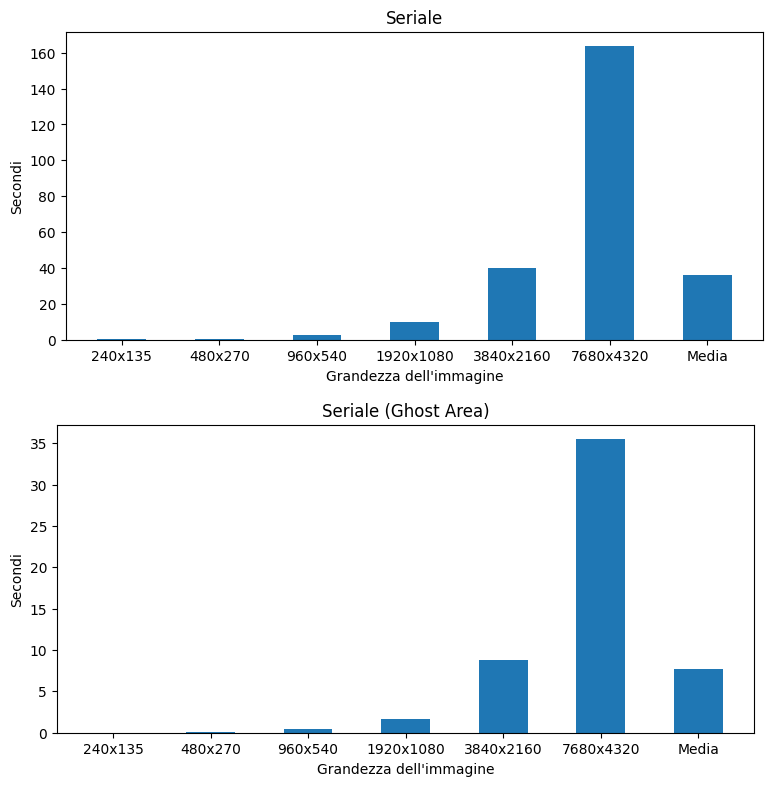
\includegraphics[width=\textwidth]{graphs_serial.png}
    \caption{I tempi di esecuzione per i programmi seriali.}
    \label{img:times_ser}
\end{figure}

\begin{figure}[h]
    \centering
    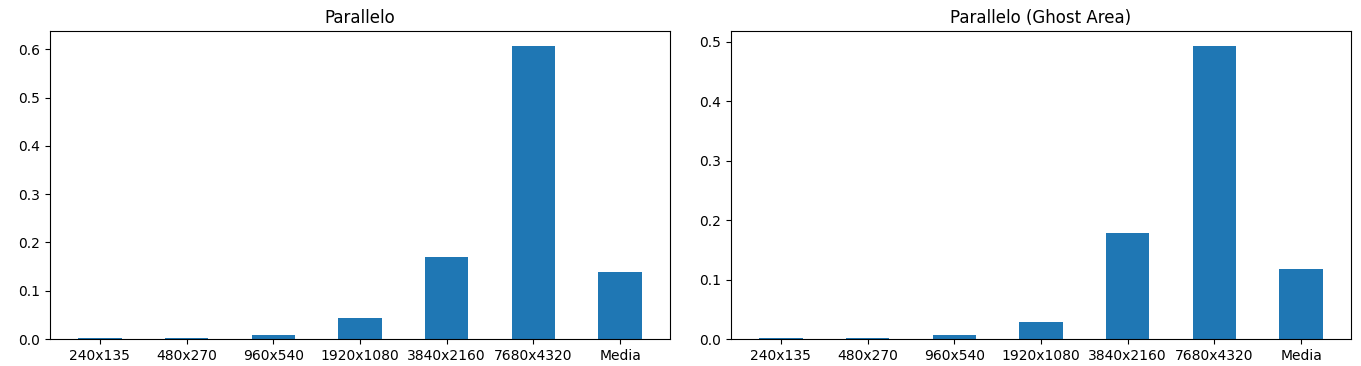
\includegraphics[width=\textwidth]{graphs_parallel.png}
    \caption{I tempi di esecuzione per i programmi paralleli.}
    \label{img:times_par}
\end{figure}

\begin{figure}[h]
    \centering
    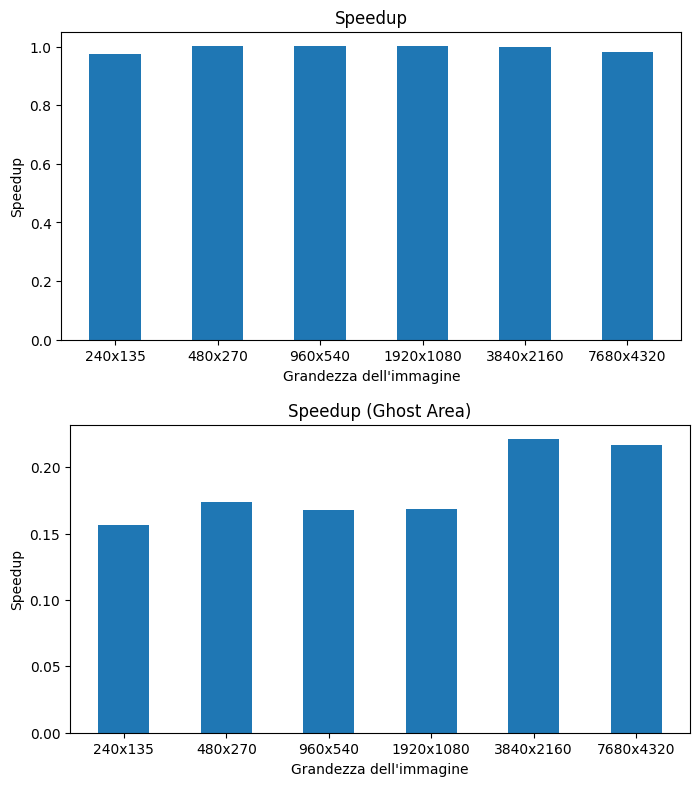
\includegraphics[width=\textwidth]{speedup.png}
    \caption[Gli Gli speedup tra i programmi seriali e paralleli.]{Gli speedup tra i programmi seriali e paralleli. Gli speedup sono tra i due programmi senza \textit{ghost area} e i due programmi con la \textit{ghost area}.}
    \label{img:speedup}
\end{figure}

\begin{figure}[h]
    \centering
    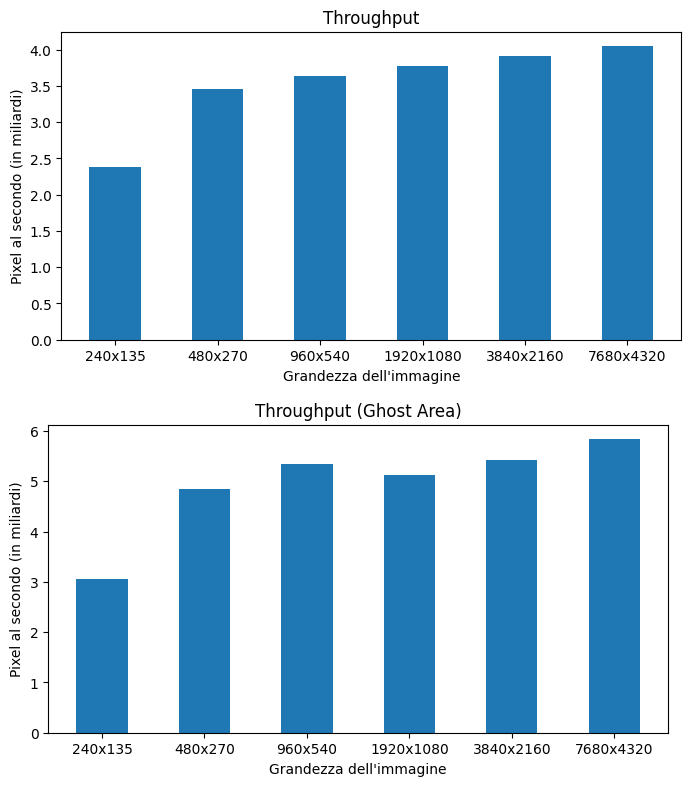
\includegraphics[width=\textwidth]{throughput.png}
    \caption{Il throughput nei due programmi paralleli.}
    \label{img:throughput}
\end{figure}

\chapter*{Conclusioni}

\rhead[\fancyplain{}{\bfseries CONCLUSIONI}]{\fancyplain{}{\bfseries\thepage}}
\lhead[\fancyplain{}{\bfseries\thepage}]{\fancyplain{}{\bfseries CONCLUSIONI}}

\addcontentsline{toc}{chapter}{Conclusioni}

In questa tesi abbiamo analizzato e tradotto un vecchio algoritmo di \textit{stereo matching} per un hardware più moderno. In particolare, abbiamo analizzato alcune delle difficoltà che si possono riscontrare in questi lavori di traduzione e abbiamo analizzato quali sono le scelte migliori da fare e le ottimizzazione che si possono applicare nell'ambito CUDA.

L'algoritmo si presta molto bene per la parallelizzazione su GPU; nonostante ciò, mentre i risultati di prestazione sono soddisfacenti, i risultati dell'algoritmo lo sono di meno, con immagini ``rumorose'' come output. In sviluppi futuri sarebbe interessante sviluppare una versione migliore dell'algoritmo e vedere come si presta alla parallelizzazione su GPU.

Un altro sviluppo interessante sarebbero ottimizzazioni più elaborate: ad esempio, si potrebbe cercare di ``compattare'' le immagini binarie create temporaneamente durante l'esecuzione dell'algoritmo, usando un solo bit per pixel invece che un byte.

\clearpage{\pagestyle{empty}\cleardoublepage}



% %%% bibliografia %%%

\rhead[\fancyplain{}{\bfseries BIBLIOGRAFIA}]{\fancyplain{}{\bfseries\thepage}}
\lhead[\fancyplain{}{\bfseries\thepage}]{\fancyplain{}{\bfseries BIBLIOGRAFIA}}

\bibliographystyle{unsrtnat}
\bibliography{biblio}{}

\addcontentsline{toc}{chapter}{Bibliografia}

\rhead[\fancyplain{}{\bfseries \leftmark}]{\fancyplain{}{\bfseries\thepage}}
\clearpage{\pagestyle{empty}\cleardoublepage}



\chapter*{Ringraziamenti}
\addcontentsline{toc}{chapter}{Ringraziamenti}
\thispagestyle{empty}

Ringrazio la mia famiglia per il sostegno e il supporto che mi hanno dato. Ringrazio anche i miei amici e i miei compagni di università, che mi hanno accompagnato e mi hanno aiutato durante questo percorso. Ringrazio infine il prof. Moreno Marzolla per avermi aiutato con questa tesi di laurea e per essere stato sempre gentile e professionale con me.

\nocite{*}

\end{document}
